\documentclass[11pt]{article}
\usepackage[small,compact]{titlesec}
\usepackage[margin=0.25in]{geometry}
\usepackage{subcaption}
\usepackage{common}
\title{\begin{center}
{\Large Practical 4: Reinforcement Learning}
\end{center}}
\author{ Baojia Tong (baojia.tong@cern.ch)\\Yuliya Dovzhenko (dovzhenko@g.harvard.edu)\\Alan Legoallec (alanlegoallec@g.harvard.edu )\\\\Public Repository: https://github.com/tongbaojia/pubcs181}
\begin{document}
\maketitle{}

\section{Data}
\paragraph{}

\section{Method}
\subsection{Fixed Policy}
\paragraph{}
There exists simple analytical solutions to this problem, if the speed change every time is not Poisson. Given this randomness nature, the solution can no longer be deterministic. However, if the gravity is large, thus the speed change could be compensated over a certain time, a simple solution could still be achieved, as shown in Figure ~\ref{FixedPolicy}. This is coded as the "$tran\_model$" function.
\begin{figure}[] 
\centering
        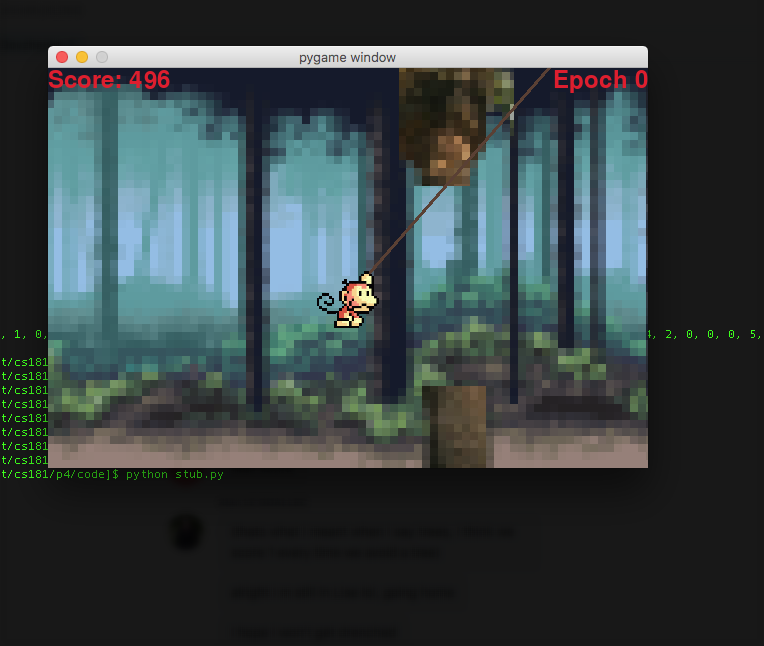
\includegraphics[width=0.33\textwidth]{Plot/highscore.png}
        \caption{In high g environment, a simple method gives an endless game; first trial can get to 496+.}
            \label{FixedPolicy}
\end{figure}

\subsection{Q-learning}
\paragraph{}
We tried off-policy method to fully explore the world.
 
\paragraph{Inputs} of this problem is the state, and the state information needs to be converted and simplified. We tried to use tree distance, monkey velocity, monkey top position and monkey-tree bottom difference to describe the state, and jump or not as action. It is worth noting that extra dimensions could be useful but also may be costly in training, since then the parameter space gets large. 

\paragraph{Initialization} is very important for this reinforcement learning. Figure ~\ref{QInitial} demonstrates that given the same variables, different initiation and binning can have very different learning behavior. Also, given the same length of game trials, a better initialization would give more reward-action iterations and hence increase the learning effect.
\begin{figure}[] 
\centering
        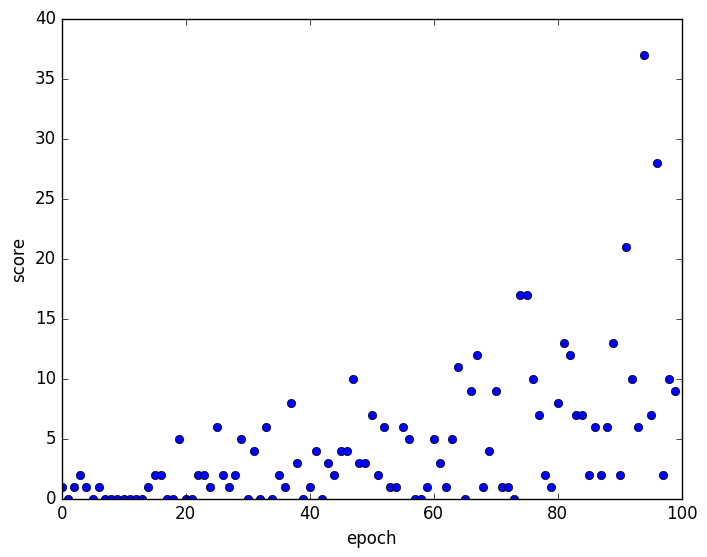
\includegraphics[width=0.33\textwidth]{Plot/learn_vel5_mtop25.png}
        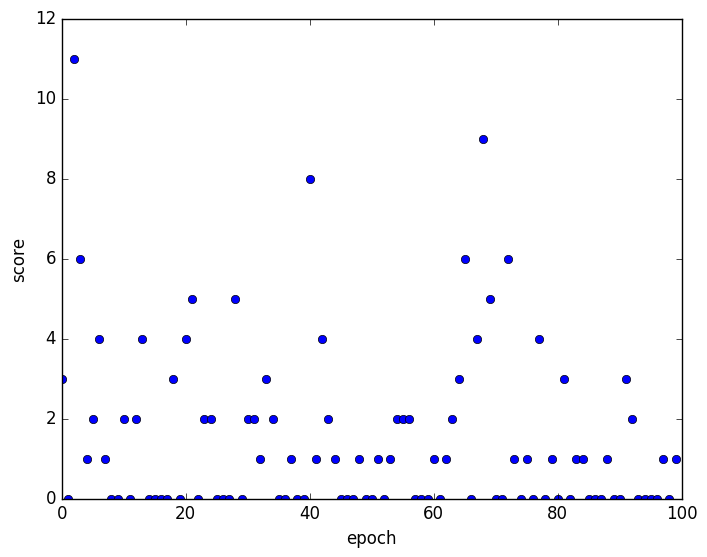
\includegraphics[width=0.33\textwidth]{Plot/learn_vel10_mtop50.png}
        \caption{In high gravity case, learning score as a function of games. Left: initialization with velocity bin size of 5 and monkey top size of 25; right: initialization with velocity bin size of 10 and monkey top size of 50.}
            \label{QInitial}
\end{figure}

\paragraph{Learning Parameters} affect the learning rate. For example, the exploration factor is described by the parameter $\epsilon$. For a larger $\epsilon$, in the early learning stage it helps to explore more states, and thus helpful for the performance. This is shown in Figure ~\ref{Qepsilon}.
\begin{figure}[] 
\centering
        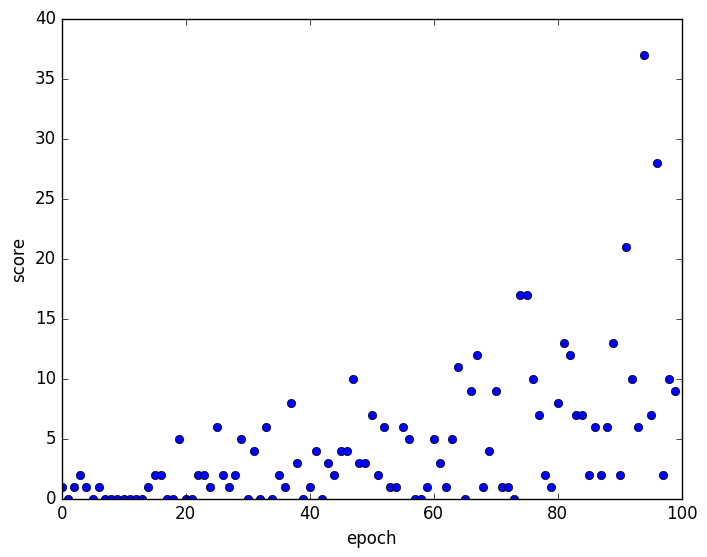
\includegraphics[width=0.33\textwidth]{Plot/learn_vel5_mtop25.png}
        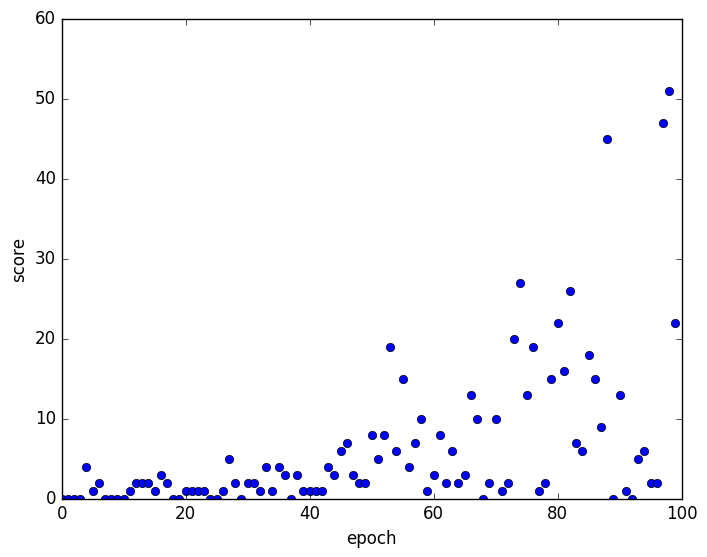
\includegraphics[width=0.33\textwidth]{Plot/learn_epsilon01.png}
        \caption{In high gravity case, learning score as a function of games. Left: initialization with $\epsilon$ of 0.001 ; right: initialization with $\epsilon$ of 0.1. Notice the y-axis increase in the larger epsilon case.}
            \label{Qepsilon}
\end{figure}


%%Tony: This paragraph could be commented out. It is very hard for me to understand this as well.
\paragraph{Modeling} for different gravity world maybe not be the same. Therefore we tried two different Q matrices, one for low gravity and one for high gravity--they have the same input parameters but different initializations. Once a new state is available, which gravity world we are in could be determined by the monkey's velocity difference. Then the corresponding Q matrix is used to learn and predict the world. In general, the low gravity case is harder to model because the randomness in the impulse will have a larger effect in the next states. This is shown in Figure ~\ref{QModel}.
\begin{figure}[] 
\centering
        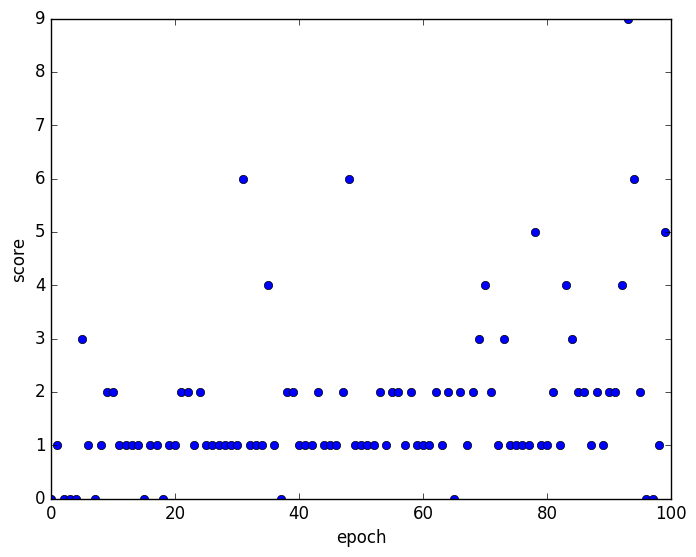
\includegraphics[width=0.3\textwidth]{Plot/learn_lowonly2.png}
        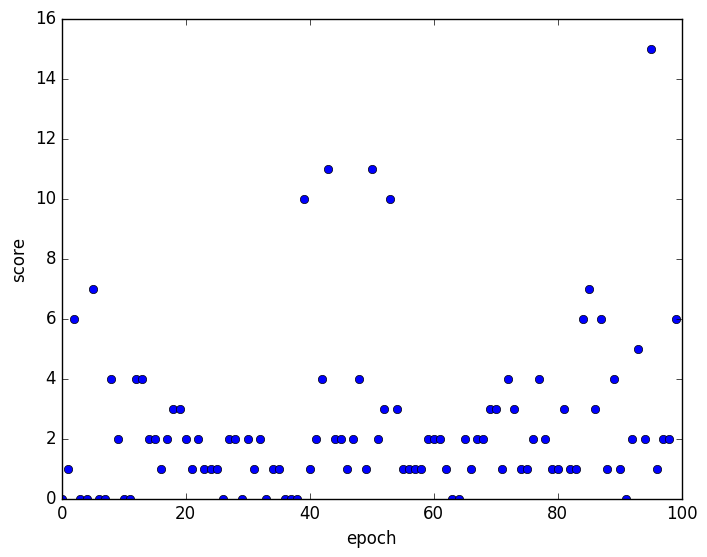
\includegraphics[width=0.3\textwidth]{Plot/learn_highonly2.png}
        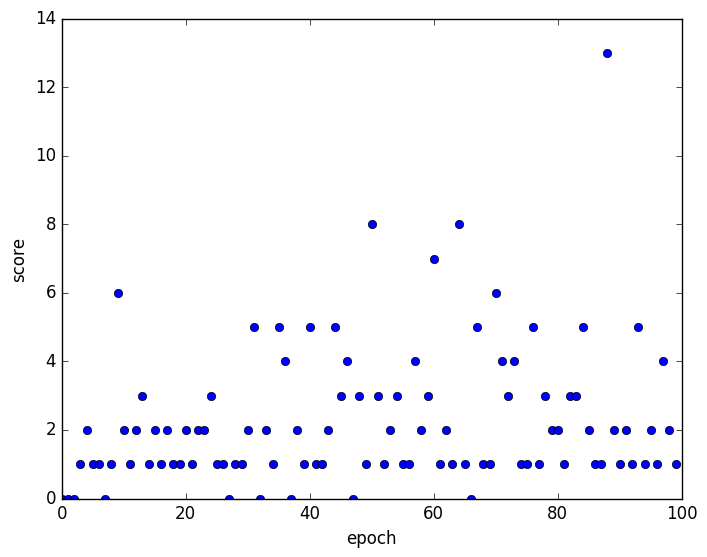
\includegraphics[width=0.3\textwidth]{Plot/learn_mix.png}
        \caption{Left: with the low G model only; middle: with the high G model only; right: with the mixed model.}
            \label{QModel}
\end{figure}

\section{Discussion} 
\paragraph{}

\end{document}

